%!TEX root = main.tex


\subsubsection{Iterated-logarithmic upper bound using a greedy 4-coloring}
We first introduce here a class of problems $I$:\\\\
$I = \{Pi = (\wdd,\bdd,W,B)\}$ where :
\begin{itemize}
    \item $\wdd = 3$
    \item $\bdd = 2$
    \item $W$ contains : $AAA,BBB,CCC$ and $|W| > 3$
    \item $B$ contains : $AB,AC,BC$
\end{itemize}
Since $\bdd = 2$ we will use the node-as-edge form.
We will now present here an algorithm $A$ that solves problems of $I$ in time $log^*n$.
\begin{itemize}
    \item We first produce a 4 labelling $A,B,C,D$ in time $log^*n$ 
    \item Then we make it greedy in the way that nodes labelled $D$ are used only when their 3 neighbors are labelled with $A,B$ and $C$
    \item White nodes colored with A label their incident edges with AAA
    \item White nodes colored with B label their incident edges with BBB
    \item White nodes colored with C label their incident edges with CCC
    \item White nodes colored with D label their incident edges with any configuration that is not $AAA$, $BBB$ or $CCC$ such that: the edge pointing towards the $A$ neighbor is not labeled $A$, the edge pointing towards the $B$ neighbor is not labeled $B$, and the edge pointing towards the $C$ neighbor is not labeled $C$.\\
\end{itemize}

\subsubsection{Iterated-logarithmic lower bound using a cover map}
\textbf{TODO Prove that an algorithm cannot do more in a tree in the LOCAL model than in the Port number \& orientation model}\\
In this section we are going to show that an algorithm must fulfill certain conditions in order to run in constant time.
Let's take an algorithm $A$ that solve $\Pi = (2,3,W,B)$ in the LOCAL model. According to \textbf{TODO}, there must be a similar algorithm $A'$ that solves as well $\Pi$ in the Port numbering model given an orientation. By contrapositive, showing that such an algorithm $A'$ does not exist would then imply that $A$ would also not exists leading $\Pi$ to have a complexity strictly higher than constant.\\\\

Since the white nodes have a degree $\wdd = 2$ we can simply consider them as edges. This leads us to trees of black nodes in which nodes with a degree 3 are considered, each of these nodes must label their ports according to $B$ and for every two such nodes $u$ and $v$, if there is an edge between them, the 2 labels of the corresponding ports must be in $W$\\
Let's assume that $A'$ does exist, we are going to show that it must fail a special kind of trees.\\
Let's define the oriented multi-graph $F_G = (V, E,\preceq)$ as in the figure  \ref{fig:cv1} :\\
\begin{figure}[htb]
    \centering
    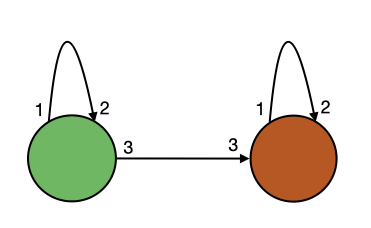
\includegraphics[scale = 0.6]{cover_map.png}
    \caption{$F_G$}
    \label{fig:cv1}
\end{figure}
Using the definitions of the chapter 8 of the textbook of Jukka Suomela \cite{3} one could easily
